% Options for packages loaded elsewhere
% Options for packages loaded elsewhere
\PassOptionsToPackage{unicode}{hyperref}
\PassOptionsToPackage{hyphens}{url}
\PassOptionsToPackage{dvipsnames,svgnames,x11names}{xcolor}
%
\documentclass[
  letterpaper,
  DIV=11,
  numbers=noendperiod]{scrreprt}
\usepackage{xcolor}
\usepackage{amsmath,amssymb}
\setcounter{secnumdepth}{5}
\usepackage{iftex}
\ifPDFTeX
  \usepackage[T1]{fontenc}
  \usepackage[utf8]{inputenc}
  \usepackage{textcomp} % provide euro and other symbols
\else % if luatex or xetex
  \usepackage{unicode-math} % this also loads fontspec
  \defaultfontfeatures{Scale=MatchLowercase}
  \defaultfontfeatures[\rmfamily]{Ligatures=TeX,Scale=1}
\fi
\usepackage{lmodern}
\ifPDFTeX\else
  % xetex/luatex font selection
\fi
% Use upquote if available, for straight quotes in verbatim environments
\IfFileExists{upquote.sty}{\usepackage{upquote}}{}
\IfFileExists{microtype.sty}{% use microtype if available
  \usepackage[]{microtype}
  \UseMicrotypeSet[protrusion]{basicmath} % disable protrusion for tt fonts
}{}
\makeatletter
\@ifundefined{KOMAClassName}{% if non-KOMA class
  \IfFileExists{parskip.sty}{%
    \usepackage{parskip}
  }{% else
    \setlength{\parindent}{0pt}
    \setlength{\parskip}{6pt plus 2pt minus 1pt}}
}{% if KOMA class
  \KOMAoptions{parskip=half}}
\makeatother
% Make \paragraph and \subparagraph free-standing
\makeatletter
\ifx\paragraph\undefined\else
  \let\oldparagraph\paragraph
  \renewcommand{\paragraph}{
    \@ifstar
      \xxxParagraphStar
      \xxxParagraphNoStar
  }
  \newcommand{\xxxParagraphStar}[1]{\oldparagraph*{#1}\mbox{}}
  \newcommand{\xxxParagraphNoStar}[1]{\oldparagraph{#1}\mbox{}}
\fi
\ifx\subparagraph\undefined\else
  \let\oldsubparagraph\subparagraph
  \renewcommand{\subparagraph}{
    \@ifstar
      \xxxSubParagraphStar
      \xxxSubParagraphNoStar
  }
  \newcommand{\xxxSubParagraphStar}[1]{\oldsubparagraph*{#1}\mbox{}}
  \newcommand{\xxxSubParagraphNoStar}[1]{\oldsubparagraph{#1}\mbox{}}
\fi
\makeatother


\usepackage{longtable,booktabs,array}
\usepackage{calc} % for calculating minipage widths
% Correct order of tables after \paragraph or \subparagraph
\usepackage{etoolbox}
\makeatletter
\patchcmd\longtable{\par}{\if@noskipsec\mbox{}\fi\par}{}{}
\makeatother
% Allow footnotes in longtable head/foot
\IfFileExists{footnotehyper.sty}{\usepackage{footnotehyper}}{\usepackage{footnote}}
\makesavenoteenv{longtable}
\usepackage{graphicx}
\makeatletter
\newsavebox\pandoc@box
\newcommand*\pandocbounded[1]{% scales image to fit in text height/width
  \sbox\pandoc@box{#1}%
  \Gscale@div\@tempa{\textheight}{\dimexpr\ht\pandoc@box+\dp\pandoc@box\relax}%
  \Gscale@div\@tempb{\linewidth}{\wd\pandoc@box}%
  \ifdim\@tempb\p@<\@tempa\p@\let\@tempa\@tempb\fi% select the smaller of both
  \ifdim\@tempa\p@<\p@\scalebox{\@tempa}{\usebox\pandoc@box}%
  \else\usebox{\pandoc@box}%
  \fi%
}
% Set default figure placement to htbp
\def\fps@figure{htbp}
\makeatother





\setlength{\emergencystretch}{3em} % prevent overfull lines

\providecommand{\tightlist}{%
  \setlength{\itemsep}{0pt}\setlength{\parskip}{0pt}}



 


\KOMAoption{captions}{tableheading}
\makeatletter
\@ifpackageloaded{bookmark}{}{\usepackage{bookmark}}
\makeatother
\makeatletter
\@ifpackageloaded{caption}{}{\usepackage{caption}}
\AtBeginDocument{%
\ifdefined\contentsname
  \renewcommand*\contentsname{Table of contents}
\else
  \newcommand\contentsname{Table of contents}
\fi
\ifdefined\listfigurename
  \renewcommand*\listfigurename{List of Figures}
\else
  \newcommand\listfigurename{List of Figures}
\fi
\ifdefined\listtablename
  \renewcommand*\listtablename{List of Tables}
\else
  \newcommand\listtablename{List of Tables}
\fi
\ifdefined\figurename
  \renewcommand*\figurename{Figure}
\else
  \newcommand\figurename{Figure}
\fi
\ifdefined\tablename
  \renewcommand*\tablename{Table}
\else
  \newcommand\tablename{Table}
\fi
}
\@ifpackageloaded{float}{}{\usepackage{float}}
\floatstyle{ruled}
\@ifundefined{c@chapter}{\newfloat{codelisting}{h}{lop}}{\newfloat{codelisting}{h}{lop}[chapter]}
\floatname{codelisting}{Listing}
\newcommand*\listoflistings{\listof{codelisting}{List of Listings}}
\makeatother
\makeatletter
\makeatother
\makeatletter
\@ifpackageloaded{caption}{}{\usepackage{caption}}
\@ifpackageloaded{subcaption}{}{\usepackage{subcaption}}
\makeatother
\usepackage{bookmark}
\IfFileExists{xurl.sty}{\usepackage{xurl}}{} % add URL line breaks if available
\urlstyle{same}
\hypersetup{
  pdftitle={My Songs for You},
  pdfauthor={Mineva Azzahra},
  colorlinks=true,
  linkcolor={blue},
  filecolor={Maroon},
  citecolor={Blue},
  urlcolor={Blue},
  pdfcreator={LaTeX via pandoc}}


\title{My Songs for You}
\usepackage{etoolbox}
\makeatletter
\providecommand{\subtitle}[1]{% add subtitle to \maketitle
  \apptocmd{\@title}{\par {\large #1 \par}}{}{}
}
\makeatother
\subtitle{Portfolio Asesmen II-2100 KIPP}
\author{Mineva Azzahra}
\date{2025-10-15}
\begin{document}
\maketitle

\renewcommand*\contentsname{Table of contents}
{
\hypersetup{linkcolor=}
\setcounter{tocdepth}{2}
\tableofcontents
}

\bookmarksetup{startatroot}

\chapter*{Hai!}\label{hai}
\addcontentsline{toc}{chapter}{Hai!}

\markboth{Hai!}{Hai!}

\begin{figure}[H]

{\centering \includegraphics[width=9.5\linewidth,height=\textheight,keepaspectratio]{images/AZRL.png}

}

\caption{About Me}

\end{figure}%

\begin{center}\rule{0.5\linewidth}{0.5pt}\end{center}

\section*{Selamat Datang! ₍\^{}. .\^{}₎⟆}\label{selamat-datang-.-.}
\addcontentsline{toc}{section}{Selamat Datang! ₍\^{}. .\^{}₎⟆}

\markright{Selamat Datang! ₍\^{}. .\^{}₎⟆}

Saya \textbf{Mineva Azzahra}, seorang mahasiswi Sistem dan Teknologi
Informasi dari Bandung.

\begin{center}\rule{0.5\linewidth}{0.5pt}\end{center}

\section*{Bingkai Berpikir: Penumpang atau
Pengemudi?}\label{bingkai-berpikir-penumpang-atau-pengemudi}
\addcontentsline{toc}{section}{Bingkai Berpikir: Penumpang atau
Pengemudi?}

\markright{Bingkai Berpikir: Penumpang atau Pengemudi?}

Dalam hidup, ada dua cara memandang perjalanan: sebagai penumpang yang
pasrah mengikuti arus, atau sebagai pengemudi yang sadar memegang
kendali. Konsep psikologis tentang \emph{Locus of Control} menyadarkan
saya bahwa keyakinan akan kendali diri bukanlah takdir, melainkan sebuah
pilihan sadar. Saya belajar bahwa merasa berdaya atau tidak berdaya
sering kali dimulai dari cara kita membingkai cerita kita sendiri.
Apakah hidup ini sesuatu yang \emph{terjadi pada saya}, atau sesuatu
yang \emph{saya jalani}?

\bookmarksetup{startatroot}

\chapter{\textgreater{} All About Me}\label{all-about-me}

\begin{figure}[H]

{\centering 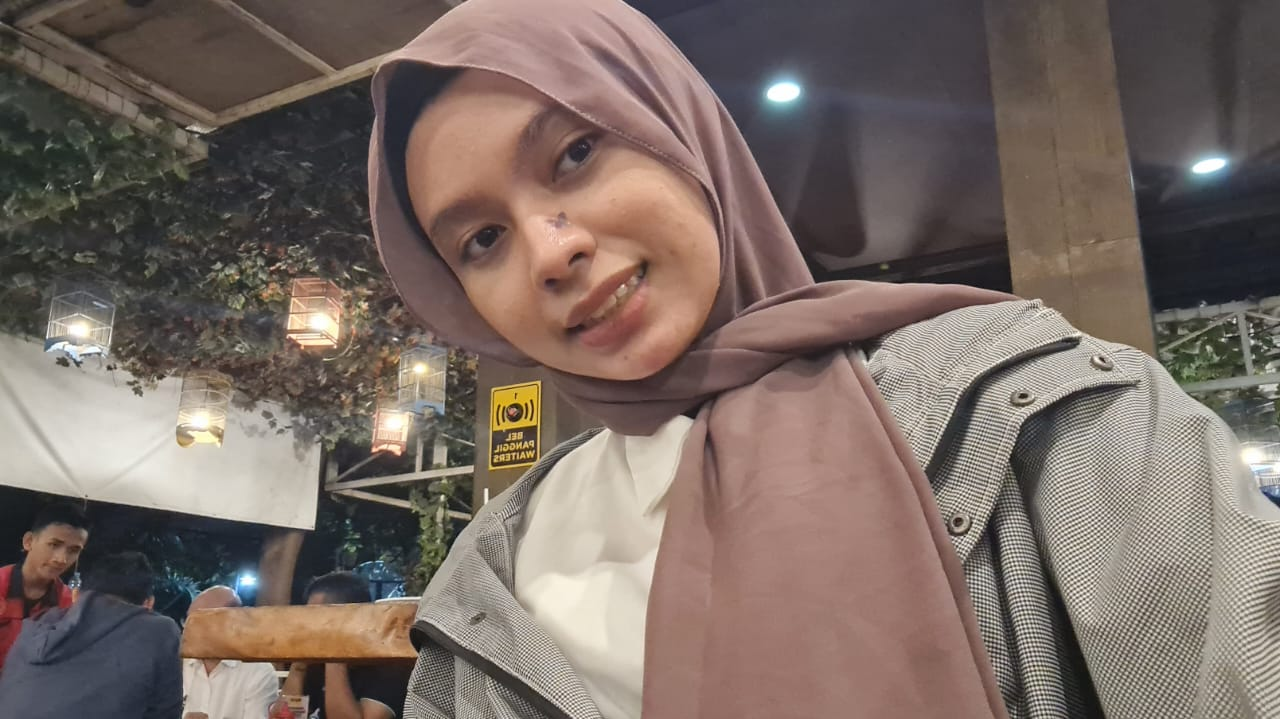
\includegraphics[width=1\linewidth,height=\textheight,keepaspectratio]{images/mi.jpeg}

}

\caption{Hello}

\end{figure}%

\begin{quote}
I am both the sun and the moon, therefore, I complete myself.
\end{quote}

\begin{center}\rule{0.5\linewidth}{0.5pt}\end{center}

\section{Selamat Datang!}\label{selamat-datang}

---to Mineva's page

Saya \textbf{\emph{Mineva Azzahra}} dan saya berasal dari
\textbf{\emph{Bandung}} (warga lokal sekitar ITB). Saya berasal dari
jurusan Sistem dan Teknologi Informasi. Mahasiswa yang percaya bahwa
setiap orang adalah sistem yang unik, dan saya bersemangat untuk
mempelajari \emph{source code} yang membentuk interaksi antarmanusia.
Jurusan ini bagi saya bukan hanya tentang belajar teknologi, tetapi juga
menjadi semacam \emph{panduan pengguna} untuk memahami dunia yang
semakin kompleks di sekitar saya.

\emph{Saya menemukan bahwa efektivitas terbaik lahir dari lingkungan
yang terstruktur, namun inovasi paling signifikan justru muncul dari
kebebasan berpikir yang tidak terikat apapun!}

\section{Sedikit Perkenalan Lagi}\label{sedikit-perkenalan-lagi}

\begin{itemize}
\tightlist
\item
  \textbf{Panggilan:} Minep/Eva/Neo
\item
  \textbf{Bahasa yang Didukung:} Indonesia (Native), Inggris (Enough),
  Sunda (Native).
\item
  \textbf{Waktu Aktif:} Paling optimal di sore dan malam hari.
\end{itemize}

\section{Fokus Pengembangan Diri}\label{fokus-pengembangan-diri}

\begin{itemize}
\tightlist
\item
  \textbf{Peningkatan Keterampilan}: Meningkatkan kompetensi di bidang
  desain (khususnya UI/UX dan desain grafis), terus memperdalam keahlian
  yang relevan dengan Sistem dan Teknologi Informasi.
\end{itemize}

\bookmarksetup{startatroot}

\chapter{\textgreater{} My Songs for You}\label{my-songs-for-you}

\begin{quote}
\emph{Songs I have personal connection with.}
\end{quote}

\section{To Life Itself?}\label{to-life-itself}

\section{Sebelah Mata}\label{sebelah-mata}

\url{https://youtu.be/u5aHyZV0CTI?si=zNwUnuZnOY9taS2E}

\begin{quote}
Tapi sebelah mataku yang lain menyadari

Gelap adalah teman setia

Dari waktu-waktu yang hilang
\end{quote}

Bukan genre lagu yang biasanya saya nikmati, tapi atmosfernya sangat
menghanyutkan. Entah mengapa ini jadi salah satu lagu yang paling sering
saya putar di tahun 2024. Jadi pengingat bahwa tidak semua hal harus
selalu ceria dan penuh semangat.

\section{For Myself}\label{for-myself}

\section{In My Mouth}\label{in-my-mouth}

\url{https://youtu.be/cIi4SxZ0IC8?si=EeUQOrJCeDpnrkRK}

\begin{quote}
I don't feel like I can be anything more than this

I don't really want to be anything more than this

I just wanna be whatever you want me to be

I don't wanna have a soul
\end{quote}

Lagu ini salah satu tipe musik yang saya sukai dan ada kenangan
tersendiri. Lagunya menyajikan ekspresi emosi yang sangat jujur dan
mentah, sulit diungkapkan dengan kata-kata biasa. Perpaduan antara lirik
yang intens tentang kehancuran diri, dan keinginan akan koneksi, dengan
musik yang abrasif, menciptakan pengalaman katarsis bagi saya sendiri.

Mendengarkan ini mungkin seperti ada di pusat badai. Tapi intinya, ada
keheningan. Semua orang bisa melewati kekacauan dalam keadaan utuh.

\emph{Kamu pusatnya, bukan korbannya}.

\section{For My Beloveds}\label{for-my-beloveds}

\subsection{Credo Quia Absurdum}\label{credo-quia-absurdum}




\end{document}
